\documentclass[11pt]{article}

    \usepackage[breakable]{tcolorbox}
    \usepackage{parskip} % Stop auto-indenting (to mimic markdown behaviour)
    

    % Basic figure setup, for now with no caption control since it's done
    % automatically by Pandoc (which extracts ![](path) syntax from Markdown).
    \usepackage{graphicx}
    % Keep aspect ratio if custom image width or height is specified
    \setkeys{Gin}{keepaspectratio}
    % Maintain compatibility with old templates. Remove in nbconvert 6.0
    \let\Oldincludegraphics\includegraphics
    % Ensure that by default, figures have no caption (until we provide a
    % proper Figure object with a Caption API and a way to capture that
    % in the conversion process - todo).
    \usepackage{caption}
    \DeclareCaptionFormat{nocaption}{}
    \captionsetup{format=nocaption,aboveskip=0pt,belowskip=0pt}

    \usepackage{float}
    \floatplacement{figure}{H} % forces figures to be placed at the correct location
    \usepackage{xcolor} % Allow colors to be defined
    \usepackage{enumerate} % Needed for markdown enumerations to work
    \usepackage{geometry} % Used to adjust the document margins
    \usepackage{amsmath} % Equations
    \usepackage{amssymb} % Equations
    \usepackage{textcomp} % defines textquotesingle
    % Hack from http://tex.stackexchange.com/a/47451/13684:
    \AtBeginDocument{%
        \def\PYZsq{\textquotesingle}% Upright quotes in Pygmentized code
    }
    \usepackage{upquote} % Upright quotes for verbatim code
    \usepackage{eurosym} % defines \euro

    \usepackage{iftex}
    \ifPDFTeX
        \usepackage[T1]{fontenc}
        \IfFileExists{alphabeta.sty}{
              \usepackage{alphabeta}
          }{
              \usepackage[mathletters]{ucs}
              \usepackage[utf8x]{inputenc}
          }
    \else
        \usepackage{fontspec}
        \usepackage{unicode-math}
    \fi

    \usepackage{fancyvrb} % verbatim replacement that allows latex
    \usepackage{grffile} % extends the file name processing of package graphics
                         % to support a larger range
    \makeatletter % fix for old versions of grffile with XeLaTeX
    \@ifpackagelater{grffile}{2019/11/01}
    {
      % Do nothing on new versions
    }
    {
      \def\Gread@@xetex#1{%
        \IfFileExists{"\Gin@base".bb}%
        {\Gread@eps{\Gin@base.bb}}%
        {\Gread@@xetex@aux#1}%
      }
    }
    \makeatother
    \usepackage[Export]{adjustbox} % Used to constrain images to a maximum size
    \adjustboxset{max size={0.9\linewidth}{0.9\paperheight}}

    % The hyperref package gives us a pdf with properly built
    % internal navigation ('pdf bookmarks' for the table of contents,
    % internal cross-reference links, web links for URLs, etc.)
    \usepackage{hyperref}
    % The default LaTeX title has an obnoxious amount of whitespace. By default,
    % titling removes some of it. It also provides customization options.
    \usepackage{titling}
    \usepackage{longtable} % longtable support required by pandoc >1.10
    \usepackage{booktabs}  % table support for pandoc > 1.12.2
    \usepackage{array}     % table support for pandoc >= 2.11.3
    \usepackage{calc}      % table minipage width calculation for pandoc >= 2.11.1
    \usepackage[inline]{enumitem} % IRkernel/repr support (it uses the enumerate* environment)
    \usepackage[normalem]{ulem} % ulem is needed to support strikethroughs (\sout)
                                % normalem makes italics be italics, not underlines
    \usepackage{soul}      % strikethrough (\st) support for pandoc >= 3.0.0
    \usepackage{mathrsfs}
    

    
    % Colors for the hyperref package
    \definecolor{urlcolor}{rgb}{0,.145,.698}
    \definecolor{linkcolor}{rgb}{.71,0.21,0.01}
    \definecolor{citecolor}{rgb}{.12,.54,.11}

    % ANSI colors
    \definecolor{ansi-black}{HTML}{3E424D}
    \definecolor{ansi-black-intense}{HTML}{282C36}
    \definecolor{ansi-red}{HTML}{E75C58}
    \definecolor{ansi-red-intense}{HTML}{B22B31}
    \definecolor{ansi-green}{HTML}{00A250}
    \definecolor{ansi-green-intense}{HTML}{007427}
    \definecolor{ansi-yellow}{HTML}{DDB62B}
    \definecolor{ansi-yellow-intense}{HTML}{B27D12}
    \definecolor{ansi-blue}{HTML}{208FFB}
    \definecolor{ansi-blue-intense}{HTML}{0065CA}
    \definecolor{ansi-magenta}{HTML}{D160C4}
    \definecolor{ansi-magenta-intense}{HTML}{A03196}
    \definecolor{ansi-cyan}{HTML}{60C6C8}
    \definecolor{ansi-cyan-intense}{HTML}{258F8F}
    \definecolor{ansi-white}{HTML}{C5C1B4}
    \definecolor{ansi-white-intense}{HTML}{A1A6B2}
    \definecolor{ansi-default-inverse-fg}{HTML}{FFFFFF}
    \definecolor{ansi-default-inverse-bg}{HTML}{000000}

    % common color for the border for error outputs.
    \definecolor{outerrorbackground}{HTML}{FFDFDF}

    % commands and environments needed by pandoc snippets
    % extracted from the output of `pandoc -s`
    \providecommand{\tightlist}{%
      \setlength{\itemsep}{0pt}\setlength{\parskip}{0pt}}
    \DefineVerbatimEnvironment{Highlighting}{Verbatim}{commandchars=\\\{\}}
    % Add ',fontsize=\small' for more characters per line
    \newenvironment{Shaded}{}{}
    \newcommand{\KeywordTok}[1]{\textcolor[rgb]{0.00,0.44,0.13}{\textbf{{#1}}}}
    \newcommand{\DataTypeTok}[1]{\textcolor[rgb]{0.56,0.13,0.00}{{#1}}}
    \newcommand{\DecValTok}[1]{\textcolor[rgb]{0.25,0.63,0.44}{{#1}}}
    \newcommand{\BaseNTok}[1]{\textcolor[rgb]{0.25,0.63,0.44}{{#1}}}
    \newcommand{\FloatTok}[1]{\textcolor[rgb]{0.25,0.63,0.44}{{#1}}}
    \newcommand{\CharTok}[1]{\textcolor[rgb]{0.25,0.44,0.63}{{#1}}}
    \newcommand{\StringTok}[1]{\textcolor[rgb]{0.25,0.44,0.63}{{#1}}}
    \newcommand{\CommentTok}[1]{\textcolor[rgb]{0.38,0.63,0.69}{\textit{{#1}}}}
    \newcommand{\OtherTok}[1]{\textcolor[rgb]{0.00,0.44,0.13}{{#1}}}
    \newcommand{\AlertTok}[1]{\textcolor[rgb]{1.00,0.00,0.00}{\textbf{{#1}}}}
    \newcommand{\FunctionTok}[1]{\textcolor[rgb]{0.02,0.16,0.49}{{#1}}}
    \newcommand{\RegionMarkerTok}[1]{{#1}}
    \newcommand{\ErrorTok}[1]{\textcolor[rgb]{1.00,0.00,0.00}{\textbf{{#1}}}}
    \newcommand{\NormalTok}[1]{{#1}}

    % Additional commands for more recent versions of Pandoc
    \newcommand{\ConstantTok}[1]{\textcolor[rgb]{0.53,0.00,0.00}{{#1}}}
    \newcommand{\SpecialCharTok}[1]{\textcolor[rgb]{0.25,0.44,0.63}{{#1}}}
    \newcommand{\VerbatimStringTok}[1]{\textcolor[rgb]{0.25,0.44,0.63}{{#1}}}
    \newcommand{\SpecialStringTok}[1]{\textcolor[rgb]{0.73,0.40,0.53}{{#1}}}
    \newcommand{\ImportTok}[1]{{#1}}
    \newcommand{\DocumentationTok}[1]{\textcolor[rgb]{0.73,0.13,0.13}{\textit{{#1}}}}
    \newcommand{\AnnotationTok}[1]{\textcolor[rgb]{0.38,0.63,0.69}{\textbf{\textit{{#1}}}}}
    \newcommand{\CommentVarTok}[1]{\textcolor[rgb]{0.38,0.63,0.69}{\textbf{\textit{{#1}}}}}
    \newcommand{\VariableTok}[1]{\textcolor[rgb]{0.10,0.09,0.49}{{#1}}}
    \newcommand{\ControlFlowTok}[1]{\textcolor[rgb]{0.00,0.44,0.13}{\textbf{{#1}}}}
    \newcommand{\OperatorTok}[1]{\textcolor[rgb]{0.40,0.40,0.40}{{#1}}}
    \newcommand{\BuiltInTok}[1]{{#1}}
    \newcommand{\ExtensionTok}[1]{{#1}}
    \newcommand{\PreprocessorTok}[1]{\textcolor[rgb]{0.74,0.48,0.00}{{#1}}}
    \newcommand{\AttributeTok}[1]{\textcolor[rgb]{0.49,0.56,0.16}{{#1}}}
    \newcommand{\InformationTok}[1]{\textcolor[rgb]{0.38,0.63,0.69}{\textbf{\textit{{#1}}}}}
    \newcommand{\WarningTok}[1]{\textcolor[rgb]{0.38,0.63,0.69}{\textbf{\textit{{#1}}}}}
    \makeatletter
    \newsavebox\pandoc@box
    \newcommand*\pandocbounded[1]{%
      \sbox\pandoc@box{#1}%
      % scaling factors for width and height
      \Gscale@div\@tempa\textheight{\dimexpr\ht\pandoc@box+\dp\pandoc@box\relax}%
      \Gscale@div\@tempb\linewidth{\wd\pandoc@box}%
      % select the smaller of both
      \ifdim\@tempb\p@<\@tempa\p@
        \let\@tempa\@tempb
      \fi
      % scaling accordingly (\@tempa < 1)
      \ifdim\@tempa\p@<\p@
        \scalebox{\@tempa}{\usebox\pandoc@box}%
      % scaling not needed, use as it is
      \else
        \usebox{\pandoc@box}%
      \fi
    }
    \makeatother

    % Define a nice break command that doesn't care if a line doesn't already
    % exist.
    \def\br{\hspace*{\fill} \\* }
    % Math Jax compatibility definitions
    \def\gt{>}
    \def\lt{<}
    \let\Oldtex\TeX
    \let\Oldlatex\LaTeX
    \renewcommand{\TeX}{\textrm{\Oldtex}}
    \renewcommand{\LaTeX}{\textrm{\Oldlatex}}
    % Document parameters
    % Document title
    \title{04\_start}
    
    
    
    
    
    
    
% Pygments definitions
\makeatletter
\def\PY@reset{\let\PY@it=\relax \let\PY@bf=\relax%
    \let\PY@ul=\relax \let\PY@tc=\relax%
    \let\PY@bc=\relax \let\PY@ff=\relax}
\def\PY@tok#1{\csname PY@tok@#1\endcsname}
\def\PY@toks#1+{\ifx\relax#1\empty\else%
    \PY@tok{#1}\expandafter\PY@toks\fi}
\def\PY@do#1{\PY@bc{\PY@tc{\PY@ul{%
    \PY@it{\PY@bf{\PY@ff{#1}}}}}}}
\def\PY#1#2{\PY@reset\PY@toks#1+\relax+\PY@do{#2}}

\@namedef{PY@tok@w}{\def\PY@tc##1{\textcolor[rgb]{0.73,0.73,0.73}{##1}}}
\@namedef{PY@tok@c}{\let\PY@it=\textit\def\PY@tc##1{\textcolor[rgb]{0.24,0.48,0.48}{##1}}}
\@namedef{PY@tok@cp}{\def\PY@tc##1{\textcolor[rgb]{0.61,0.40,0.00}{##1}}}
\@namedef{PY@tok@k}{\let\PY@bf=\textbf\def\PY@tc##1{\textcolor[rgb]{0.00,0.50,0.00}{##1}}}
\@namedef{PY@tok@kp}{\def\PY@tc##1{\textcolor[rgb]{0.00,0.50,0.00}{##1}}}
\@namedef{PY@tok@kt}{\def\PY@tc##1{\textcolor[rgb]{0.69,0.00,0.25}{##1}}}
\@namedef{PY@tok@o}{\def\PY@tc##1{\textcolor[rgb]{0.40,0.40,0.40}{##1}}}
\@namedef{PY@tok@ow}{\let\PY@bf=\textbf\def\PY@tc##1{\textcolor[rgb]{0.67,0.13,1.00}{##1}}}
\@namedef{PY@tok@nb}{\def\PY@tc##1{\textcolor[rgb]{0.00,0.50,0.00}{##1}}}
\@namedef{PY@tok@nf}{\def\PY@tc##1{\textcolor[rgb]{0.00,0.00,1.00}{##1}}}
\@namedef{PY@tok@nc}{\let\PY@bf=\textbf\def\PY@tc##1{\textcolor[rgb]{0.00,0.00,1.00}{##1}}}
\@namedef{PY@tok@nn}{\let\PY@bf=\textbf\def\PY@tc##1{\textcolor[rgb]{0.00,0.00,1.00}{##1}}}
\@namedef{PY@tok@ne}{\let\PY@bf=\textbf\def\PY@tc##1{\textcolor[rgb]{0.80,0.25,0.22}{##1}}}
\@namedef{PY@tok@nv}{\def\PY@tc##1{\textcolor[rgb]{0.10,0.09,0.49}{##1}}}
\@namedef{PY@tok@no}{\def\PY@tc##1{\textcolor[rgb]{0.53,0.00,0.00}{##1}}}
\@namedef{PY@tok@nl}{\def\PY@tc##1{\textcolor[rgb]{0.46,0.46,0.00}{##1}}}
\@namedef{PY@tok@ni}{\let\PY@bf=\textbf\def\PY@tc##1{\textcolor[rgb]{0.44,0.44,0.44}{##1}}}
\@namedef{PY@tok@na}{\def\PY@tc##1{\textcolor[rgb]{0.41,0.47,0.13}{##1}}}
\@namedef{PY@tok@nt}{\let\PY@bf=\textbf\def\PY@tc##1{\textcolor[rgb]{0.00,0.50,0.00}{##1}}}
\@namedef{PY@tok@nd}{\def\PY@tc##1{\textcolor[rgb]{0.67,0.13,1.00}{##1}}}
\@namedef{PY@tok@s}{\def\PY@tc##1{\textcolor[rgb]{0.73,0.13,0.13}{##1}}}
\@namedef{PY@tok@sd}{\let\PY@it=\textit\def\PY@tc##1{\textcolor[rgb]{0.73,0.13,0.13}{##1}}}
\@namedef{PY@tok@si}{\let\PY@bf=\textbf\def\PY@tc##1{\textcolor[rgb]{0.64,0.35,0.47}{##1}}}
\@namedef{PY@tok@se}{\let\PY@bf=\textbf\def\PY@tc##1{\textcolor[rgb]{0.67,0.36,0.12}{##1}}}
\@namedef{PY@tok@sr}{\def\PY@tc##1{\textcolor[rgb]{0.64,0.35,0.47}{##1}}}
\@namedef{PY@tok@ss}{\def\PY@tc##1{\textcolor[rgb]{0.10,0.09,0.49}{##1}}}
\@namedef{PY@tok@sx}{\def\PY@tc##1{\textcolor[rgb]{0.00,0.50,0.00}{##1}}}
\@namedef{PY@tok@m}{\def\PY@tc##1{\textcolor[rgb]{0.40,0.40,0.40}{##1}}}
\@namedef{PY@tok@gh}{\let\PY@bf=\textbf\def\PY@tc##1{\textcolor[rgb]{0.00,0.00,0.50}{##1}}}
\@namedef{PY@tok@gu}{\let\PY@bf=\textbf\def\PY@tc##1{\textcolor[rgb]{0.50,0.00,0.50}{##1}}}
\@namedef{PY@tok@gd}{\def\PY@tc##1{\textcolor[rgb]{0.63,0.00,0.00}{##1}}}
\@namedef{PY@tok@gi}{\def\PY@tc##1{\textcolor[rgb]{0.00,0.52,0.00}{##1}}}
\@namedef{PY@tok@gr}{\def\PY@tc##1{\textcolor[rgb]{0.89,0.00,0.00}{##1}}}
\@namedef{PY@tok@ge}{\let\PY@it=\textit}
\@namedef{PY@tok@gs}{\let\PY@bf=\textbf}
\@namedef{PY@tok@ges}{\let\PY@bf=\textbf\let\PY@it=\textit}
\@namedef{PY@tok@gp}{\let\PY@bf=\textbf\def\PY@tc##1{\textcolor[rgb]{0.00,0.00,0.50}{##1}}}
\@namedef{PY@tok@go}{\def\PY@tc##1{\textcolor[rgb]{0.44,0.44,0.44}{##1}}}
\@namedef{PY@tok@gt}{\def\PY@tc##1{\textcolor[rgb]{0.00,0.27,0.87}{##1}}}
\@namedef{PY@tok@err}{\def\PY@bc##1{{\setlength{\fboxsep}{\string -\fboxrule}\fcolorbox[rgb]{1.00,0.00,0.00}{1,1,1}{\strut ##1}}}}
\@namedef{PY@tok@kc}{\let\PY@bf=\textbf\def\PY@tc##1{\textcolor[rgb]{0.00,0.50,0.00}{##1}}}
\@namedef{PY@tok@kd}{\let\PY@bf=\textbf\def\PY@tc##1{\textcolor[rgb]{0.00,0.50,0.00}{##1}}}
\@namedef{PY@tok@kn}{\let\PY@bf=\textbf\def\PY@tc##1{\textcolor[rgb]{0.00,0.50,0.00}{##1}}}
\@namedef{PY@tok@kr}{\let\PY@bf=\textbf\def\PY@tc##1{\textcolor[rgb]{0.00,0.50,0.00}{##1}}}
\@namedef{PY@tok@bp}{\def\PY@tc##1{\textcolor[rgb]{0.00,0.50,0.00}{##1}}}
\@namedef{PY@tok@fm}{\def\PY@tc##1{\textcolor[rgb]{0.00,0.00,1.00}{##1}}}
\@namedef{PY@tok@vc}{\def\PY@tc##1{\textcolor[rgb]{0.10,0.09,0.49}{##1}}}
\@namedef{PY@tok@vg}{\def\PY@tc##1{\textcolor[rgb]{0.10,0.09,0.49}{##1}}}
\@namedef{PY@tok@vi}{\def\PY@tc##1{\textcolor[rgb]{0.10,0.09,0.49}{##1}}}
\@namedef{PY@tok@vm}{\def\PY@tc##1{\textcolor[rgb]{0.10,0.09,0.49}{##1}}}
\@namedef{PY@tok@sa}{\def\PY@tc##1{\textcolor[rgb]{0.73,0.13,0.13}{##1}}}
\@namedef{PY@tok@sb}{\def\PY@tc##1{\textcolor[rgb]{0.73,0.13,0.13}{##1}}}
\@namedef{PY@tok@sc}{\def\PY@tc##1{\textcolor[rgb]{0.73,0.13,0.13}{##1}}}
\@namedef{PY@tok@dl}{\def\PY@tc##1{\textcolor[rgb]{0.73,0.13,0.13}{##1}}}
\@namedef{PY@tok@s2}{\def\PY@tc##1{\textcolor[rgb]{0.73,0.13,0.13}{##1}}}
\@namedef{PY@tok@sh}{\def\PY@tc##1{\textcolor[rgb]{0.73,0.13,0.13}{##1}}}
\@namedef{PY@tok@s1}{\def\PY@tc##1{\textcolor[rgb]{0.73,0.13,0.13}{##1}}}
\@namedef{PY@tok@mb}{\def\PY@tc##1{\textcolor[rgb]{0.40,0.40,0.40}{##1}}}
\@namedef{PY@tok@mf}{\def\PY@tc##1{\textcolor[rgb]{0.40,0.40,0.40}{##1}}}
\@namedef{PY@tok@mh}{\def\PY@tc##1{\textcolor[rgb]{0.40,0.40,0.40}{##1}}}
\@namedef{PY@tok@mi}{\def\PY@tc##1{\textcolor[rgb]{0.40,0.40,0.40}{##1}}}
\@namedef{PY@tok@il}{\def\PY@tc##1{\textcolor[rgb]{0.40,0.40,0.40}{##1}}}
\@namedef{PY@tok@mo}{\def\PY@tc##1{\textcolor[rgb]{0.40,0.40,0.40}{##1}}}
\@namedef{PY@tok@ch}{\let\PY@it=\textit\def\PY@tc##1{\textcolor[rgb]{0.24,0.48,0.48}{##1}}}
\@namedef{PY@tok@cm}{\let\PY@it=\textit\def\PY@tc##1{\textcolor[rgb]{0.24,0.48,0.48}{##1}}}
\@namedef{PY@tok@cpf}{\let\PY@it=\textit\def\PY@tc##1{\textcolor[rgb]{0.24,0.48,0.48}{##1}}}
\@namedef{PY@tok@c1}{\let\PY@it=\textit\def\PY@tc##1{\textcolor[rgb]{0.24,0.48,0.48}{##1}}}
\@namedef{PY@tok@cs}{\let\PY@it=\textit\def\PY@tc##1{\textcolor[rgb]{0.24,0.48,0.48}{##1}}}

\def\PYZbs{\char`\\}
\def\PYZus{\char`\_}
\def\PYZob{\char`\{}
\def\PYZcb{\char`\}}
\def\PYZca{\char`\^}
\def\PYZam{\char`\&}
\def\PYZlt{\char`\<}
\def\PYZgt{\char`\>}
\def\PYZsh{\char`\#}
\def\PYZpc{\char`\%}
\def\PYZdl{\char`\$}
\def\PYZhy{\char`\-}
\def\PYZsq{\char`\'}
\def\PYZdq{\char`\"}
\def\PYZti{\char`\~}
% for compatibility with earlier versions
\def\PYZat{@}
\def\PYZlb{[}
\def\PYZrb{]}
\makeatother


    % For linebreaks inside Verbatim environment from package fancyvrb.
    \makeatletter
        \newbox\Wrappedcontinuationbox
        \newbox\Wrappedvisiblespacebox
        \newcommand*\Wrappedvisiblespace {\textcolor{red}{\textvisiblespace}}
        \newcommand*\Wrappedcontinuationsymbol {\textcolor{red}{\llap{\tiny$\m@th\hookrightarrow$}}}
        \newcommand*\Wrappedcontinuationindent {3ex }
        \newcommand*\Wrappedafterbreak {\kern\Wrappedcontinuationindent\copy\Wrappedcontinuationbox}
        % Take advantage of the already applied Pygments mark-up to insert
        % potential linebreaks for TeX processing.
        %        {, <, #, %, $, ' and ": go to next line.
        %        _, }, ^, &, >, - and ~: stay at end of broken line.
        % Use of \textquotesingle for straight quote.
        \newcommand*\Wrappedbreaksatspecials {%
            \def\PYGZus{\discretionary{\char`\_}{\Wrappedafterbreak}{\char`\_}}%
            \def\PYGZob{\discretionary{}{\Wrappedafterbreak\char`\{}{\char`\{}}%
            \def\PYGZcb{\discretionary{\char`\}}{\Wrappedafterbreak}{\char`\}}}%
            \def\PYGZca{\discretionary{\char`\^}{\Wrappedafterbreak}{\char`\^}}%
            \def\PYGZam{\discretionary{\char`\&}{\Wrappedafterbreak}{\char`\&}}%
            \def\PYGZlt{\discretionary{}{\Wrappedafterbreak\char`\<}{\char`\<}}%
            \def\PYGZgt{\discretionary{\char`\>}{\Wrappedafterbreak}{\char`\>}}%
            \def\PYGZsh{\discretionary{}{\Wrappedafterbreak\char`\#}{\char`\#}}%
            \def\PYGZpc{\discretionary{}{\Wrappedafterbreak\char`\%}{\char`\%}}%
            \def\PYGZdl{\discretionary{}{\Wrappedafterbreak\char`\$}{\char`\$}}%
            \def\PYGZhy{\discretionary{\char`\-}{\Wrappedafterbreak}{\char`\-}}%
            \def\PYGZsq{\discretionary{}{\Wrappedafterbreak\textquotesingle}{\textquotesingle}}%
            \def\PYGZdq{\discretionary{}{\Wrappedafterbreak\char`\"}{\char`\"}}%
            \def\PYGZti{\discretionary{\char`\~}{\Wrappedafterbreak}{\char`\~}}%
        }
        % Some characters . , ; ? ! / are not pygmentized.
        % This macro makes them "active" and they will insert potential linebreaks
        \newcommand*\Wrappedbreaksatpunct {%
            \lccode`\~`\.\lowercase{\def~}{\discretionary{\hbox{\char`\.}}{\Wrappedafterbreak}{\hbox{\char`\.}}}%
            \lccode`\~`\,\lowercase{\def~}{\discretionary{\hbox{\char`\,}}{\Wrappedafterbreak}{\hbox{\char`\,}}}%
            \lccode`\~`\;\lowercase{\def~}{\discretionary{\hbox{\char`\;}}{\Wrappedafterbreak}{\hbox{\char`\;}}}%
            \lccode`\~`\:\lowercase{\def~}{\discretionary{\hbox{\char`\:}}{\Wrappedafterbreak}{\hbox{\char`\:}}}%
            \lccode`\~`\?\lowercase{\def~}{\discretionary{\hbox{\char`\?}}{\Wrappedafterbreak}{\hbox{\char`\?}}}%
            \lccode`\~`\!\lowercase{\def~}{\discretionary{\hbox{\char`\!}}{\Wrappedafterbreak}{\hbox{\char`\!}}}%
            \lccode`\~`\/\lowercase{\def~}{\discretionary{\hbox{\char`\/}}{\Wrappedafterbreak}{\hbox{\char`\/}}}%
            \catcode`\.\active
            \catcode`\,\active
            \catcode`\;\active
            \catcode`\:\active
            \catcode`\?\active
            \catcode`\!\active
            \catcode`\/\active
            \lccode`\~`\~
        }
    \makeatother

    \let\OriginalVerbatim=\Verbatim
    \makeatletter
    \renewcommand{\Verbatim}[1][1]{%
        %\parskip\z@skip
        \sbox\Wrappedcontinuationbox {\Wrappedcontinuationsymbol}%
        \sbox\Wrappedvisiblespacebox {\FV@SetupFont\Wrappedvisiblespace}%
        \def\FancyVerbFormatLine ##1{\hsize\linewidth
            \vtop{\raggedright\hyphenpenalty\z@\exhyphenpenalty\z@
                \doublehyphendemerits\z@\finalhyphendemerits\z@
                \strut ##1\strut}%
        }%
        % If the linebreak is at a space, the latter will be displayed as visible
        % space at end of first line, and a continuation symbol starts next line.
        % Stretch/shrink are however usually zero for typewriter font.
        \def\FV@Space {%
            \nobreak\hskip\z@ plus\fontdimen3\font minus\fontdimen4\font
            \discretionary{\copy\Wrappedvisiblespacebox}{\Wrappedafterbreak}
            {\kern\fontdimen2\font}%
        }%

        % Allow breaks at special characters using \PYG... macros.
        \Wrappedbreaksatspecials
        % Breaks at punctuation characters . , ; ? ! and / need catcode=\active
        \OriginalVerbatim[#1,codes*=\Wrappedbreaksatpunct]%
    }
    \makeatother

    % Exact colors from NB
    \definecolor{incolor}{HTML}{303F9F}
    \definecolor{outcolor}{HTML}{D84315}
    \definecolor{cellborder}{HTML}{CFCFCF}
    \definecolor{cellbackground}{HTML}{F7F7F7}

    % prompt
    \makeatletter
    \newcommand{\boxspacing}{\kern\kvtcb@left@rule\kern\kvtcb@boxsep}
    \makeatother
    \newcommand{\prompt}[4]{
        {\ttfamily\llap{{\color{#2}[#3]:\hspace{3pt}#4}}\vspace{-\baselineskip}}
    }
    

    
    % Prevent overflowing lines due to hard-to-break entities
    \sloppy
    % Setup hyperref package
    \hypersetup{
      breaklinks=true,  % so long urls are correctly broken across lines
      colorlinks=true,
      urlcolor=urlcolor,
      linkcolor=linkcolor,
      citecolor=citecolor,
      }
    % Slightly bigger margins than the latex defaults
    
    \geometry{verbose,tmargin=1in,bmargin=1in,lmargin=1in,rmargin=1in}
    
    

\begin{document}
    
    \maketitle
    
    

    
    \section{Week 4 - Why does fluid drag complicate
things?}\label{week-4---why-does-fluid-drag-complicate-things}

As an object moves through the fluid, the molecules of the fluid collide
with the object and exert a force on it. This collision changes the
momentum oof the object just a little bit. The collision does so in a
random way, but the average effect of all those collisions is to exert a
force on the object that is proportional to a function of the object's
velocity, \(F(v)\). In some cases those collisions occur such that they
make an impact; other times they might approach the object more slowly
and slide over it in a more frictional interaction. These two behaviors
are both fluid drag, but they are different forms.

The first form (\(F \sim v^2\)) describes the behavior of things like a
skydiver falling, a high-speed car, or a baseball thrown through the
air. But it can also be valid for the movement of fish in water, or a
submarine moving through the ocean. Through those collisions, the
distribution of those forces can cause intra-body forces, which can
result in damage or deformation of the object. However, we often model
the body as solid and focus on the way this form of air resistance
changes the motion.

This form of air resistance cannot describe the behavior of objects
approaching the speed of sound in the fluid. Objects moving a speeds
that high can produce
\href{https://en.wikipedia.org/wiki/Shock_wave}{shock fronts} that
forces the fluid to go through abrupt changes in density, pressure, and
temperature. Below is a figure of a shock front produced the nose of a
jet flying at supersonic speeds.

\begin{figure}
\centering
\pandocbounded{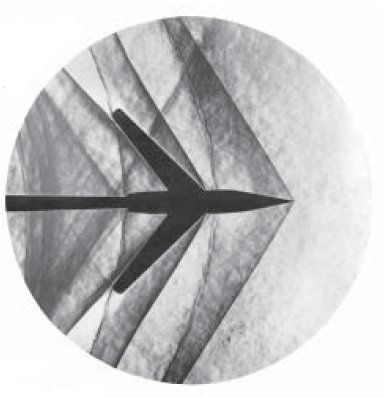
\includegraphics[keepaspectratio,alt={A shock front from a supersonic jet}]{/Users/caballero/repos/teaching/modern-classical-mechanics/images/notes/week4/shock_front.jpg}}
\caption{A shock front from a supersonic jet}
\end{figure}

The second form (\(F \sim v\)) describes the flow of a viscous fluid
around a solid object. You might think of this as pulling an object
through some viscous oil, honey, or even molasses. The movement of the
fluid around the object exerts a force and slows the motion of the
object. In water, this form can explain the motion of some of the
smallest creatures on Earth, like the
\href{https://en.wikipedia.org/wiki/Tardigrade}{water bear}, an amoeba,
or a paramecium.

What is interesting here is that these creatures have had to adapt to
this form of fluid drag.
\href{https://en.wikipedia.org/wiki/Edward_M._Purcell}{Edward Purcell}
wrote a paper in 1977 called
\href{../../docs/papers/purcell_AJP_1977.pdf}{Life at Low Reynolds
Number} that describes the motion of these creatures. He demonstrates
that the physics in this regime requires creature to have adapted forms
of locomotion that can take advantage of that environment.

\subsection{Why do we often neglect air
resistance?}\label{why-do-we-often-neglect-air-resistance}

We're in the business of making models of physical systems using the
concepts and tools of Classical Mechanics. We've focused on Newton's
Laws, which are a formulation of mechanics that starts from the concept
of the force.

We often start with that approach because the mathematical tools that we
have available to us when we are first learning physics are geometry and
algebra. Forces are a vector concept and Newton's Second Law is a vector
equation that holds in each of the three dimensions of space. This
formulation lends itself to a decomposing problems often into two or
three separate problems, one for each dimension, and then using some
algebra to solve the problems. However, that mathematics limits the
kinds of explorations we can do.

This is one reason why we neglect
\href{https://en.wikipedia.org/wiki/Air_resistance}{air resistance} in
our first explorations of motion. Our models of air resistance are more
complicated and require more advanced mathematics to solve. The
equations of motion can be coupled and non-linear. In some cases, we
cannot solve the equations of motion analytically and must resort to
numerical methods like
\href{https://en.wikipedia.org/wiki/Euler_method}{Euler's method}, or
the more often used
\href{https://en.wikipedia.org/wiki/Runge\%E2\%80\%93Kutta_methods}{Runge-Kutta
method}.

    \subsection{The Reynolds Number}\label{the-reynolds-number}

The different forms of fluid drag are often described by a dimensionless
number called the
\href{https://en.wikipedia.org/wiki/Reynolds_number}{Reynolds Number}.
The Reynolds number is a ratio of the inertial forces to the viscous
forces in a fluid.

\begin{itemize}
\tightlist
\item
  What are inertial forces? They are the ones associated with resistance
  to motion, the mass of the object. The more massive the object in a
  given setup, the higher the inertial contribution.
\item
  What are viscous forces? They are the ones associated with the
  interaction of the fluid with the object. The more viscous the fluid -
  the harder it for is to flow under the same conditions, the higher the
  viscous contribution.
\end{itemize}

The Reynolds number is defined as:

\[Re = \frac{\rho v L}{\mu}\]

where \(\rho\) is the density of the fluid, \(v\) is the velocity of the
object in that fluid, \(L\) is a characteristic length of the object,
and \(\mu\) is the dynamic viscosity of the fluid.

You can probably see who the Reynolds number characterizes the system of
the object and the fluid as their are properties of both the object and
the fluid in the equation. The Reynolds number can be measured quite
accurately in a lab because the laboratory setups are typically designed
to make the measurement of the Reynolds number easier. We will often
estimate it in theoretical physics.

\subsubsection{What is a characteristic
length?}\label{what-is-a-characteristic-length}

This length is a generic length scale associated with the flow, this can
be the order of magnitude size of the object, or, in the absence of an
object, the same for the pipe or channel in which the flow is occurring.
If it's an airplane, it can be the wingspan, or the length of the
fuselage. If it's a car, it can be the length of the car. If it's a
sphere, it can be the radius, and so on.

\subsubsection{What is dynamic
viscosity?}\label{what-is-dynamic-viscosity}

Viscosity is the measure of the fluid's resistance to flow. It's how the
fluid slides past itself. It's a bit of a harder quantity to describe,
but you can think of it as the ``stickiness'' of the fluid. The higher
the viscosity, the more sticky the fluid is -- really, for a given
setup, the more viscous fluid will flow more slowly. The lower the
viscosity, the higher tendency for a fluid to flow. Compare honey to
water in the same vessel and temperature, and you'll observe the
difference in viscosity.

\paragraph{Measuring viscosity}\label{measuring-viscosity}

We can sometimes measure viscosity with a
\href{https://en.wikipedia.org/wiki/Viscometer}{viscometer}, which uses
a \href{https://en.wikipedia.org/wiki/Capillary_tube}{capillary tube} to
measure the time it takes for a fluid to flow through a tube of known
dimensions. However, this works best for
\href{https://en.wikipedia.org/wiki/Newtonian_fluid}{Newtonian fluids},
which are fluids that have a constant viscosity.

\paragraph{Non-Newtonian fluids (in your
kitchen)}\label{non-newtonian-fluids-in-your-kitchen}

Not all fluids are Newtonian, and some fluids have a viscosity that
changes with the rate of flow. These
\href{https://en.wikipedia.org/wiki/Non-Newtonian_fluid}{non-Newtonian
fluids} can be \href{https://en.wikipedia.org/wiki/Shear_thinning}{shear
thinning} or \href{https://en.wikipedia.org/wiki/Shear_thickening}{shear
thickening}. Shear thinning fluids become less viscous when they are
stirred or shaken, while shear thickening fluids become more viscous
when they are stirred or shaken.

Below is a video from
\href{https://www.americastestkitchen.com/}{America's Test Kitchen} that
demonstrates the behavior of a non-Newtonian fluid. The fluid is made
from cornstarch and water, and it's called
\href{https://en.wikipedia.org/wiki/Oobleck}{oobleck}.

\href{https://youtube.com/watch?v=FrLh1GILomc}{\pandocbounded{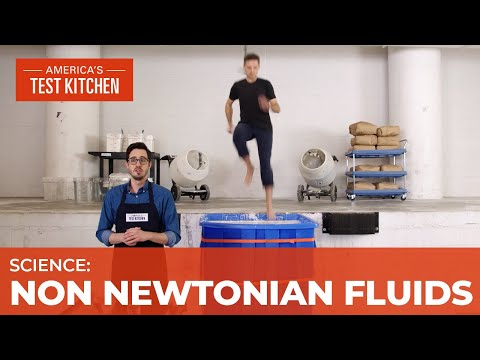
\includegraphics[keepaspectratio,alt={America's Test Kitchen Non-Newtonian Fluids}]{/Users/caballero/repos/teaching/modern-classical-mechanics/images/notes/week4/FrLh1GILomc.jpg}}}

Source: \url{https://www.youtube.com/watch?v=FrLh1GILomc}

The physics of cooking is fascinating and covers the field of
\href{https://en.wikipedia.org/wiki/Soft_matter}{soft matter physics}.
There's a free course on the subject offered by
\href{https://pll.harvard.edu/course/science-cooking-haute-cuisine-soft-matter-science-physics}{Harvard
and EdX}.

    \subsubsection{Low Reynolds Number
Flows}\label{low-reynolds-number-flows}

A low Reynolds number flow is a flow where the viscous forces dominate
the inertial forces. The object is moving slowly, or the fluid is very
viscous, or the object is very small. We typically think of these flows
as being in the range of \(Re < 1\). In these flows, the motion of the
fluid is typically laminar; it flows in fairly smooth and parallel
layers. Low Reynolds number flows can produce dynamics that is
counterintutive. Below are a couple videos that explain the physics of
low Reynolds number flows.

\paragraph{Physics of Life - Life at Low Reynolds Number (15 minute
video)}\label{physics-of-life---life-at-low-reynolds-number-15-minute-video}

This video focuses on the biological aspects of the problem as the
physics of low Reynolds numbers is important for understanding the
motion of microorganisms.

\href{https://youtube.com/watch?v=gZk2bMaqs1E}{\pandocbounded{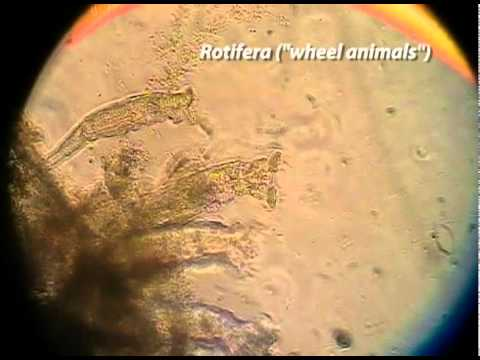
\includegraphics[keepaspectratio,alt={Physics of Life - Life at Low Reynolds Number}]{/Users/caballero/repos/teaching/modern-classical-mechanics/images/notes/week4/gZk2bMaqs1E.jpg}})}

Source: \url{https://youtube.com/watch?v=gZk2bMaqs1E}

\paragraph{G.I. Taylor's Low Reynolds Number Flows (32 minute
video)}\label{g.i.-taylors-low-reynolds-number-flows-32-minute-video}

This video is a classic from
\href{https://en.wikipedia.org/wiki/Geoffrey_Ingram_Taylor}{G.I. Taylor}
who was a physicist interested in sharing the conceptual beauty of
physics with the general public. He was also a pioneer in the field of
fluid mechanics. In fact, Taylor's
\href{../../docs/papers/taylor_1922.pdf}{groundbreaking paper} on the
stability of fluid flows between two rotating cylinders set off studies
into turbulence. The
\href{https://en.wikipedia.org/wiki/Taylor\%E2\%80\%93Couette_flow}{Taylor-Couette
flow} is a critical tool for
\href{https://pubmed.ncbi.nlm.nih.gov/20365623/}{studies of turbulence}.

\href{https://youtube.com/watch?v=8Dst6V4CQME}{\pandocbounded{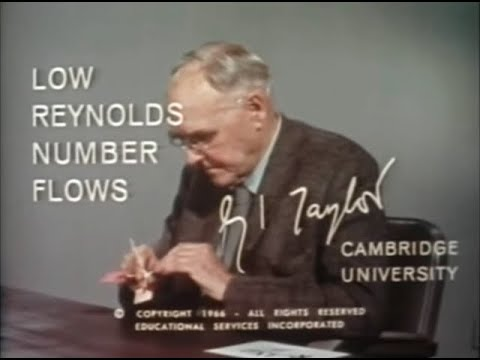
\includegraphics[keepaspectratio,alt={G.I. Taylor's Low Reynolds Number Flows}]{/Users/caballero/repos/teaching/modern-classical-mechanics/images/notes/week4/8Dst6V4CQME.jpg}}}

Source: \url{https://youtube.com/watch?v=8Dst6V4CQME}

    \subsubsection{High Reynolds Number
Flows}\label{high-reynolds-number-flows}

In high Reynolds number flows, the inertial forces dominate the viscous
forces. The object is moving quickly, or the fluid is not very viscous,
or the object is very large. We typically think of these flows as being
in the range of \(Re > 1000\). In these flows, the motion of the fluid
is typically \href{https://en.wikipedia.org/wiki/Turbulence}{turbulent}.
Turbulent flows are characterized by chaotic and irregular motion. The
fluid moves in a complex and unpredictable way, with eddies and vortices
forming and dissipating. Turbulent flows can be very difficult to
predict and model, but they are also very common in nature.

\paragraph{Von Kármán's Vortex Street (2 minute
video)}\label{von-kuxe1rmuxe1ns-vortex-street-2-minute-video}

The
\href{https://en.wikipedia.org/wiki/Von_K\%C3\%A1rm\%C3\%A1n_vortex_street}{von
Kármán vortex street} is a pattern of alternating vortices that can form
when a fluid flows past a ``bluff'' body, such as a cylinder or a
sphere. The vortices are shed from the body in a regular pattern,
creating a repeating pattern of alternating vortices. The von Kármán
vortex street is an example of a high Reynolds number flow, and it can
be used to study the behavior of turbulent flows. Below is a video of a
von Kármán vortex street simulation.

\href{https://youtube.com/watch?v=f3LmjJ1N7YE}{\pandocbounded{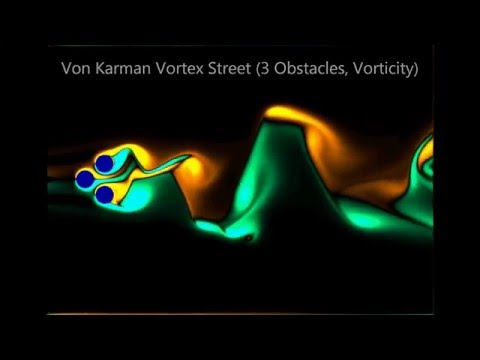
\includegraphics[keepaspectratio,alt={Von Karman's Vortex Street}]{/Users/caballero/repos/teaching/modern-classical-mechanics/images/notes/week4/f3LmjJ1N7YE.jpg}}}

Source: \url{https://youtube.com/watch?v=f3LmjJ1N7YE}

\paragraph{Turbulent Flow (24 minute
video)}\label{turbulent-flow-24-minute-video}

Turbulence is a major research area in science. We don't fully
understand it. We are trying to determine what triggers it, how to
control it, and how to predict if and when it will occur. The problem of
turbulence is frequently multi-scale such that behavior at one time or
length scale is not well explained or connected to another scale.
Additionally, the mathematics of turbulence is very difficult. It makes
for an interesting and challenging research area. Below is a video that
explains the some of the physics of turbulence. The first 4 minutes or
so are at least worth watching.

\href{https://youtube.com/watch?v=RkewD966Y90}{\pandocbounded{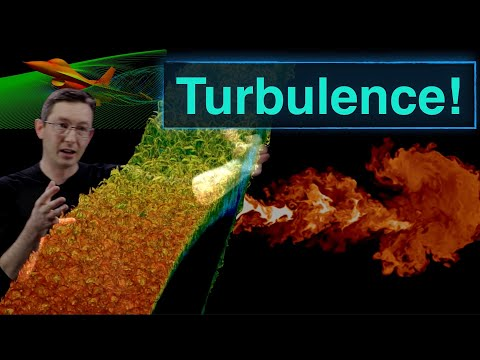
\includegraphics[keepaspectratio,alt={Turbulence}]{/Users/caballero/repos/teaching/modern-classical-mechanics/images/notes/week4/RkewD966Y90.jpg}}}

Source: \url{https://youtube.com/watch?v=RkewD966Y90}

    


    % Add a bibliography block to the postdoc
    
    
    
\end{document}
